\question \textbf{The Viterbi algorithm}

The Viterbi algorithm is a dynamic programming based method to find the optimal path of an HMM with hidden status.

\begin{figure}[H]
      \centering
      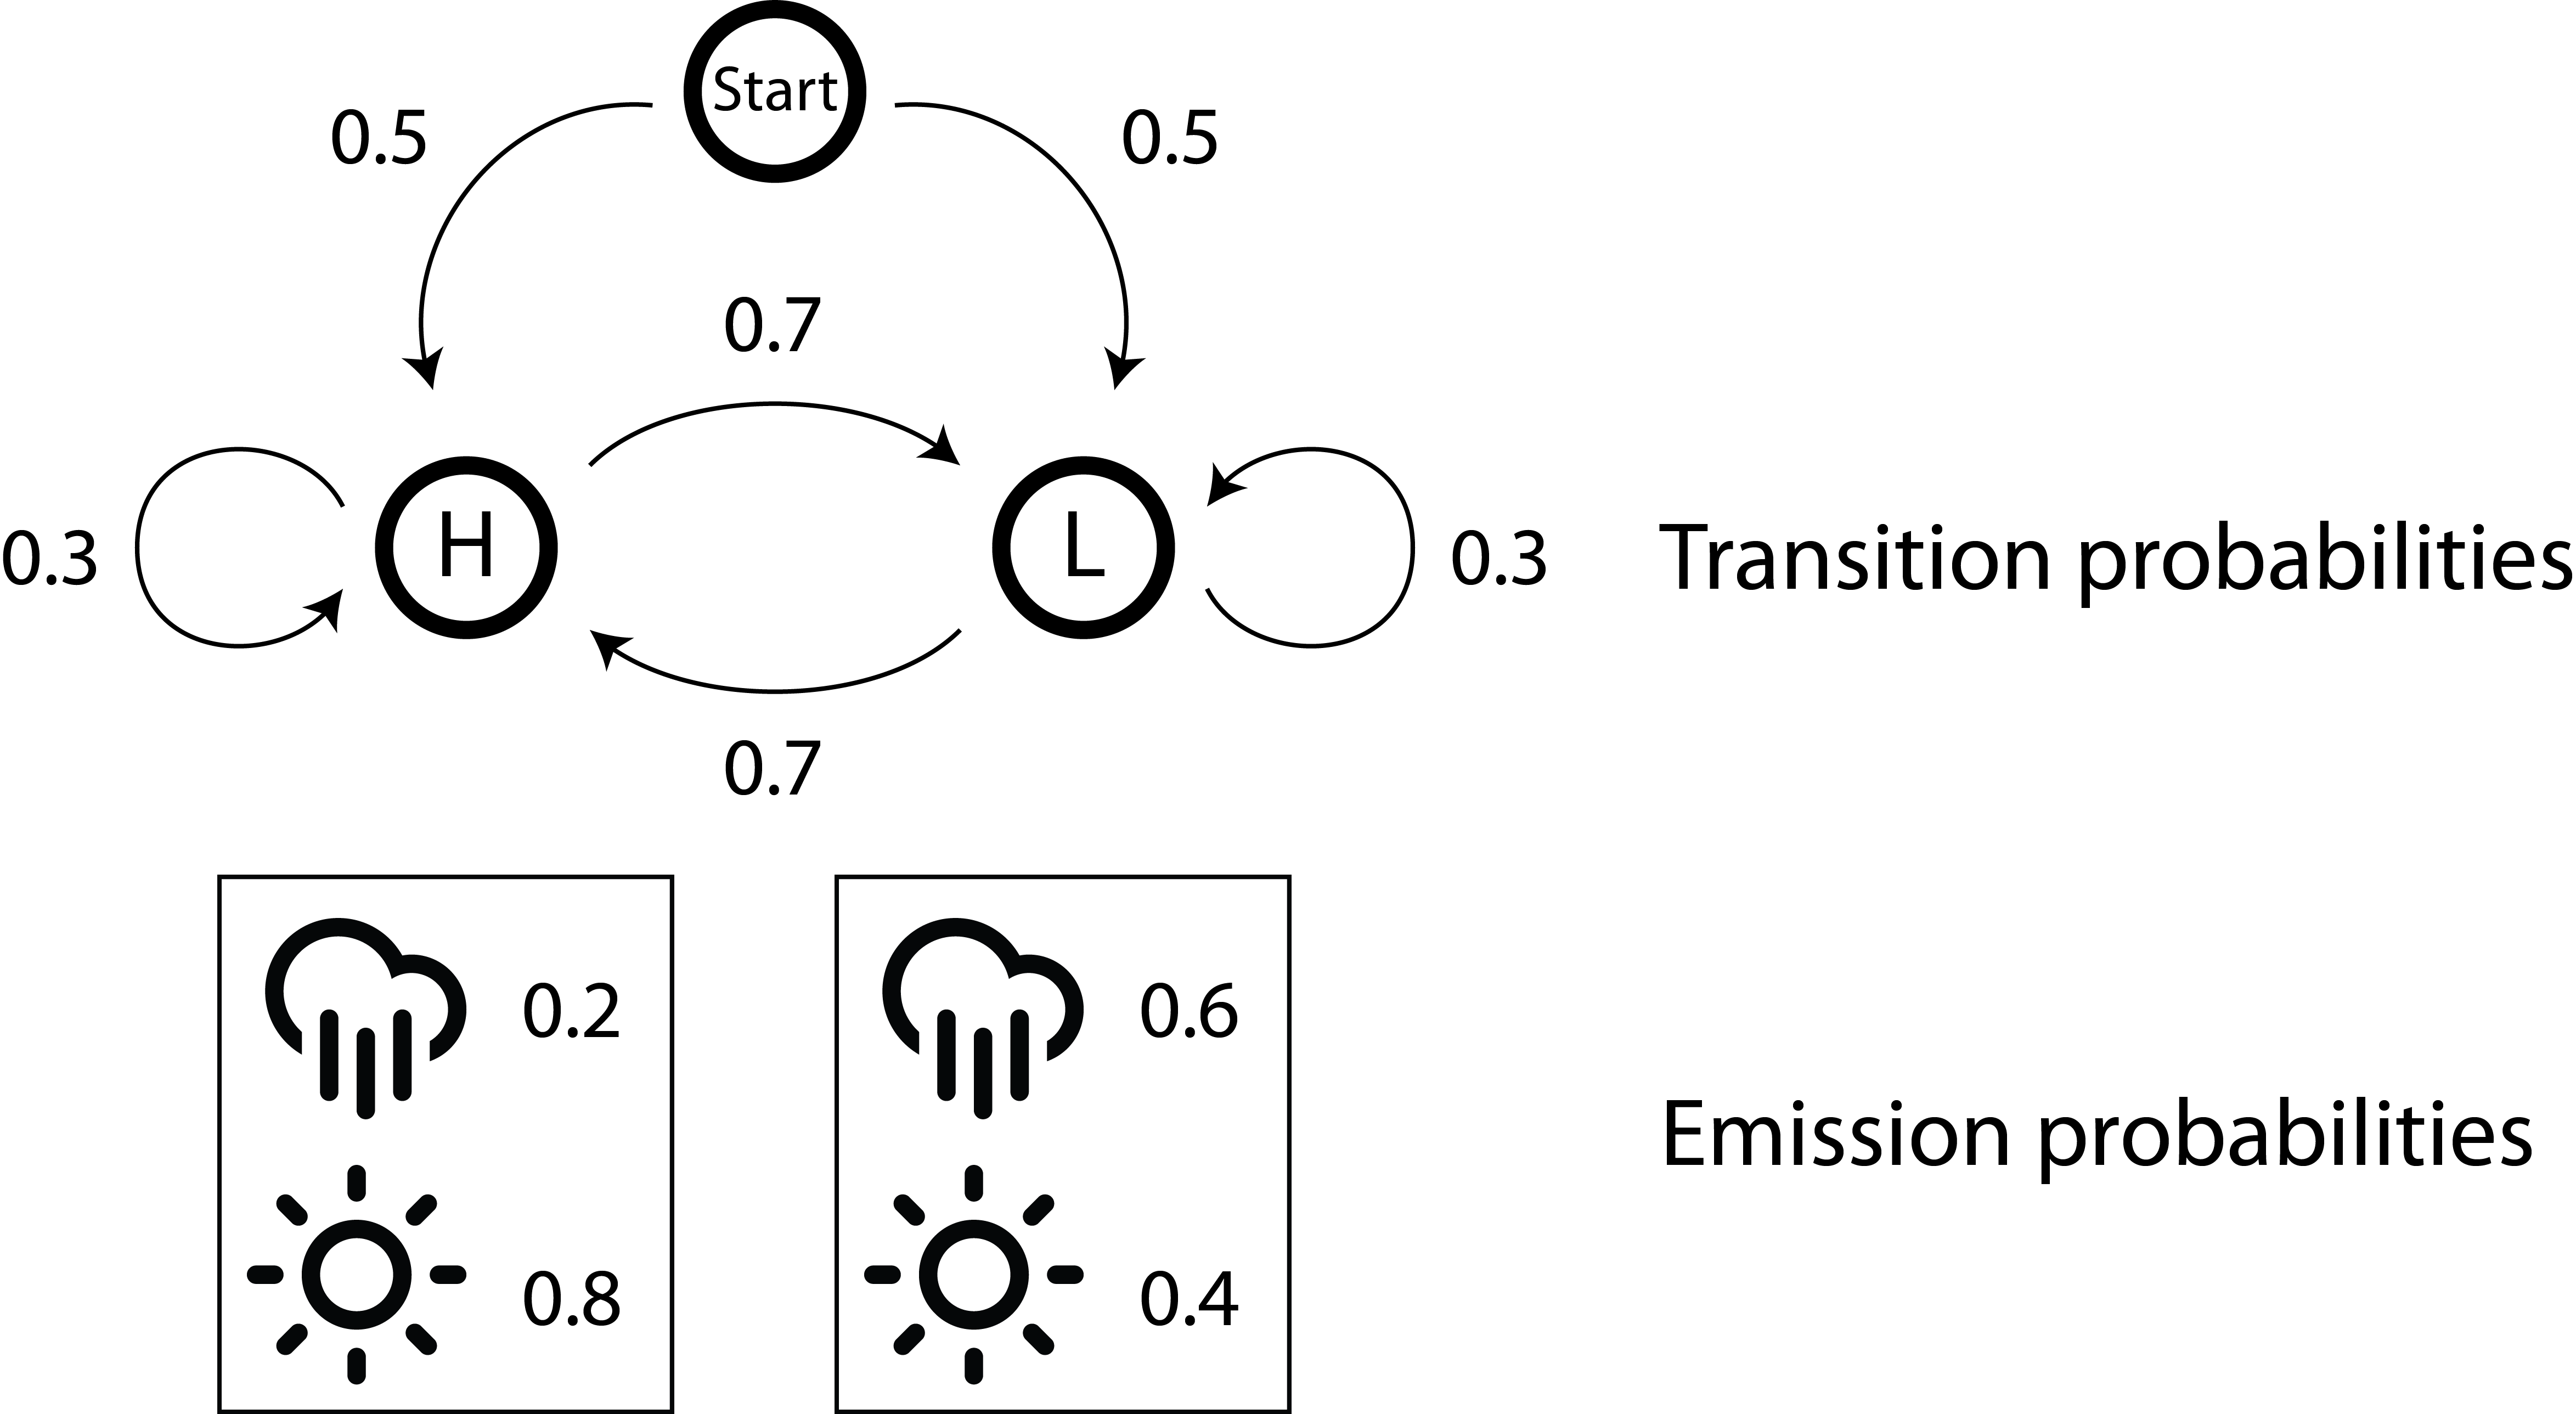
\includegraphics[width=0.6 \textwidth]{fig13/hmm_viterbi.png}
\end{figure}

\vspace{0.1 in}

\begin{parts}

%% (a)
  \part Find the optimal path when observed weather conditions are (Rain, Sunny).
\begin{table}[H]
\centering
\begin{tabular}{|c|l|l|}
\hline
                           & H                                             & L                                             \\ \hline
Rain   & \cellcolor[HTML]{CCE5FF}  $0.5 \times 0.2 = 0.1$ & \cellcolor[HTML]{CCE5FF} $0.5 \times 0.6 = 0.3$ \\ \hline
Sunny & \cellcolor[HTML]{CCE5FF}  (H) $0.1 \times 0.3 \times 0.8 = 0.024$  
           & \cellcolor[HTML]{CCE5FF} (H) $0.1 \times 0.7 \times 0.4 = 0.028$ \\
          & \cellcolor[HTML]{CCE5FF}  (L) $0.3 \times 0.7 \times 0.8 = 0.168$  
          & \cellcolor[HTML]{CCE5FF} (L) $0.3 \times 0.3 \times 0.4 = 0.036$ \\ \hline
\end{tabular}
\end{table}

\begin{solution}[0.35 in]
(L, H)
\end{solution}

%% (b)
  \part Find the optimal path when observed weather conditions are (Sunny, Sunny, Rain).
\begin{table}[H]
\centering
\begin{tabular}{|c|l|l|}
\hline
                           & H                                             & L                                             \\ \hline
Sunny & \cellcolor[HTML]{CCE5FF} $0.5 \times 0.8 = 0.4$  & \cellcolor[HTML]{CCE5FF} $0.5 \times 0.4 = 0.2$ \\ \hline
Sunny & \cellcolor[HTML]{CCE5FF}   (H) $0.4 \times 0.3 \times 0.8 = 0.096$ 
          & \cellcolor[HTML]{CCE5FF} (H) $0.4 \times 0.7 \times 0.4 = 0.112$  \\ 
          & \cellcolor[HTML]{CCE5FF}   (L) $0.2 \times 0.7 \times 0.8 = 0.112$ 
          & \cellcolor[HTML]{CCE5FF} (L) $0.2 \times 0.3 \times 0.4 = 0.024$ \\ \hline
Rain   &  \cellcolor[HTML]{CCE5FF}   (H) $0.112 \times 0.3 \times 0.2 = 0.007$ 
          & \cellcolor[HTML]{CCE5FF} (H) $0.112 \times 0.7 \times 0.6 = 0.047$ \\ 
         &  \cellcolor[HTML]{CCE5FF}    (L) $0.112 \times 0.7 \times 0.2 = 0.016$ 
         & \cellcolor[HTML]{CCE5FF} (L) $0.112 \times 0.3 \times 0.6 = 0.02$ \\ \hline
\end{tabular}
\end{table}

\begin{solution}[0.35 in]
(L, H, L)
\end{solution}

\end{parts}
